\documentclass[12pt]{ctexart}

% 导入代码块
\usepackage{listings}
\usepackage{xcolor}
\usepackage{geometry}
\usepackage{amsmath}
\usepackage{graphicx}
\usepackage{float} 
\usepackage{subfigure}




\newcommand\keywords[1]{\textbf{关键词}: #1}

% 自定义代码块样式
\lstset{
    basicstyle          =   \sffamily,          % 基本代码风格
    keywordstyle        =   \bfseries,          % 关键字风格
    commentstyle        =   \rmfamily\itshape,  % 注释的风格，斜体
    stringstyle         =   \ttfamily,  % 字符串风格
    flexiblecolumns,                % 别问为什么，加上这个
    numbers             =   left,   % 行号的位置在左边
    showspaces          =   false,  % 是否显示空格，显示了有点乱，所以不现实了
    numberstyle         =   \zihao{-5}\ttfamily,    % 行号的样式，小五号，tt等宽字体
    showstringspaces    =   false,
    captionpos          =   t,      % 这段代码的名字所呈现的位置，t指的是top上面
    frame               =   lrtb,   % 显示边框
}

\lstdefinestyle{Python}{
    language        =   Python, % 语言选Python
    basicstyle      =   \zihao{-5}\ttfamily,
    numberstyle     =   \zihao{-5}\ttfamily,
    keywordstyle    =   \color{blue},
    keywordstyle    =   [2] \color{teal},
    stringstyle     =   \color{magenta},
    commentstyle    =   \color{red}\ttfamily,
    breaklines      =   true,   % 自动换行，建议不要写太长的行
    columns         =   fixed,  % 如果不加这一句，字间距就不固定，很丑，必须加
    basewidth       =   0.5em,
}
\renewenvironment{abstract}
 {% 如果你的正文使用的是normalsize,则这里不需要这行
  \bfseries % 可选：如果你想要摘要标题加粗
  \noindent\textbf{摘要:}\quad\ignorespaces}
 {\medskip}

\geometry{a4paper,left=2.5cm,right=2.5cm,top=3cm,bottom=2.5cm,headsep=6mm,foot=10mm,twoside,bindingoffset=1cm}%定义页面

\begin{document}

\title{基于YOLOv8的鸟类识别改进方案} 
\author{1120253612 \and 莫天皓}
\date{\today} 
\maketitle 

\begin{center}
  {\Large \textbf{摘\quad 要}}
\end{center}
\vspace{1em}
鸟类识别作为生物多样性监测、生态学研究和野生动物保护的关键技术，对推动智慧生态与可持续发展具有重要意义。
针对细粒度鸟类目标检测任务中现有的模型存在的小目标漏检严重、背景干扰强以及类内差异大、类间差异小等问题，
本文提出了一种轻量高效的改进模型——YOLOv8s-Birds。该模型以YOLOv8s为基础网络进行改进，进行了三项针对鸟类识别任务的优化：
第一，将主干网络 Backbone 替换为全局上下文建模能力更强的 EfficientViT\cite{ref6} ，以增强对鸟类非局部判别性部件的关联感知；
第二，在原有特征金字塔网络 Neck 的多尺度融合过程中嵌入 CBAM\cite{ref7} 双重注意力机制，可以有效聚焦于关键局部区域并缓解复杂背景干扰的问题；
第三，引入对比学习预训练策略\cite{ref12}，利用规模更大的 iNaturalist 数据集\cite{ref11}，使用自监督信号提升模型在小样本数据集上的泛化能力。
在CUB-200-2011细粒度鸟类数据集上的实验结果表明，改进后的模型相较于原始的 YOLOv8s，在精确率（Precision）、召回率（Recall）、mAP50 和 mAP50-95 四项核心指标上均取得了显著提升，验证了所提方案的有效性与先进性。
本研究为资源受限场景下的高精度细粒度目标检测提供了一种可行的技术路径。\\
\noindent \textbf{关键词}：细粒度鸟类识别；YOLOv8；EfficientViT；CBAM注意力机制；对比学习

\newpage



\section{背景与现状分析}

\subsection{实际意义}
鸟类识别是动物检测任务中的一个重要研究方向，不论是观鸟爱好者识别鸟类，还是在保护生物多样性等方面都具有重要意义。
传统的鸟类识别需要依靠人类的肉眼识别与观察记录，再在名录上进行查询，这种方法效率低下且错误率极高。
但近年来深度学习技术与计算机视觉技术的发展，使用深度学习网络进行鸟类识别已经逐渐成为主流方法。

同时将构建的鸟类识别系统部署在野外或机场等设施周边，不但可以监视生物多样性、记录种群数量，
可以与其他设施形成联动，避免撞鸟等因鸟类引发的安全事故。


\subsection{主流模型的优缺点}

近年来，YOLO（You Only Look Once）系列目标检测算法被广泛应用于野生动物识别任务。

其具以下优点：

1. 算法简洁且识别速度快。YOLO模型是单阶段推理模型，具有较好的精确度和较小的参数量，其可以部署在野外的移动设备上。\cite{ref1}。

2. 避免背景对识别造成的影响。YOLO算法是对整张图片进行卷积, 所以对于检测目标具有更大的视野, 
因此不容易对背景误判。在鸟类识别这一背景复杂多样的任务中具有显著优势。\cite{ref2}

但是针对鸟类识别这一具体任务，简单的YOLO网络还具有很多不足：

1. 对于成群聚类的小物体, YOLO算法的表现会不如人意。部分个体较小的鸟类会有群聚的习性，所以对它们进行目标检测时会有一定的困难。\cite{ref2,ref5}

2. 类内差异大，类间差异小。同一类鸟因为季节性别等等因素，可能存在显著的差异，如图1(a)(b)。但是不同鸟类之间的的区别可能会特别轻微，
如图1(a)(c)。\cite{ref3}

\begin{figure}[htbp]
   \centering
   \subfigure[未成年体夜鹭]{
       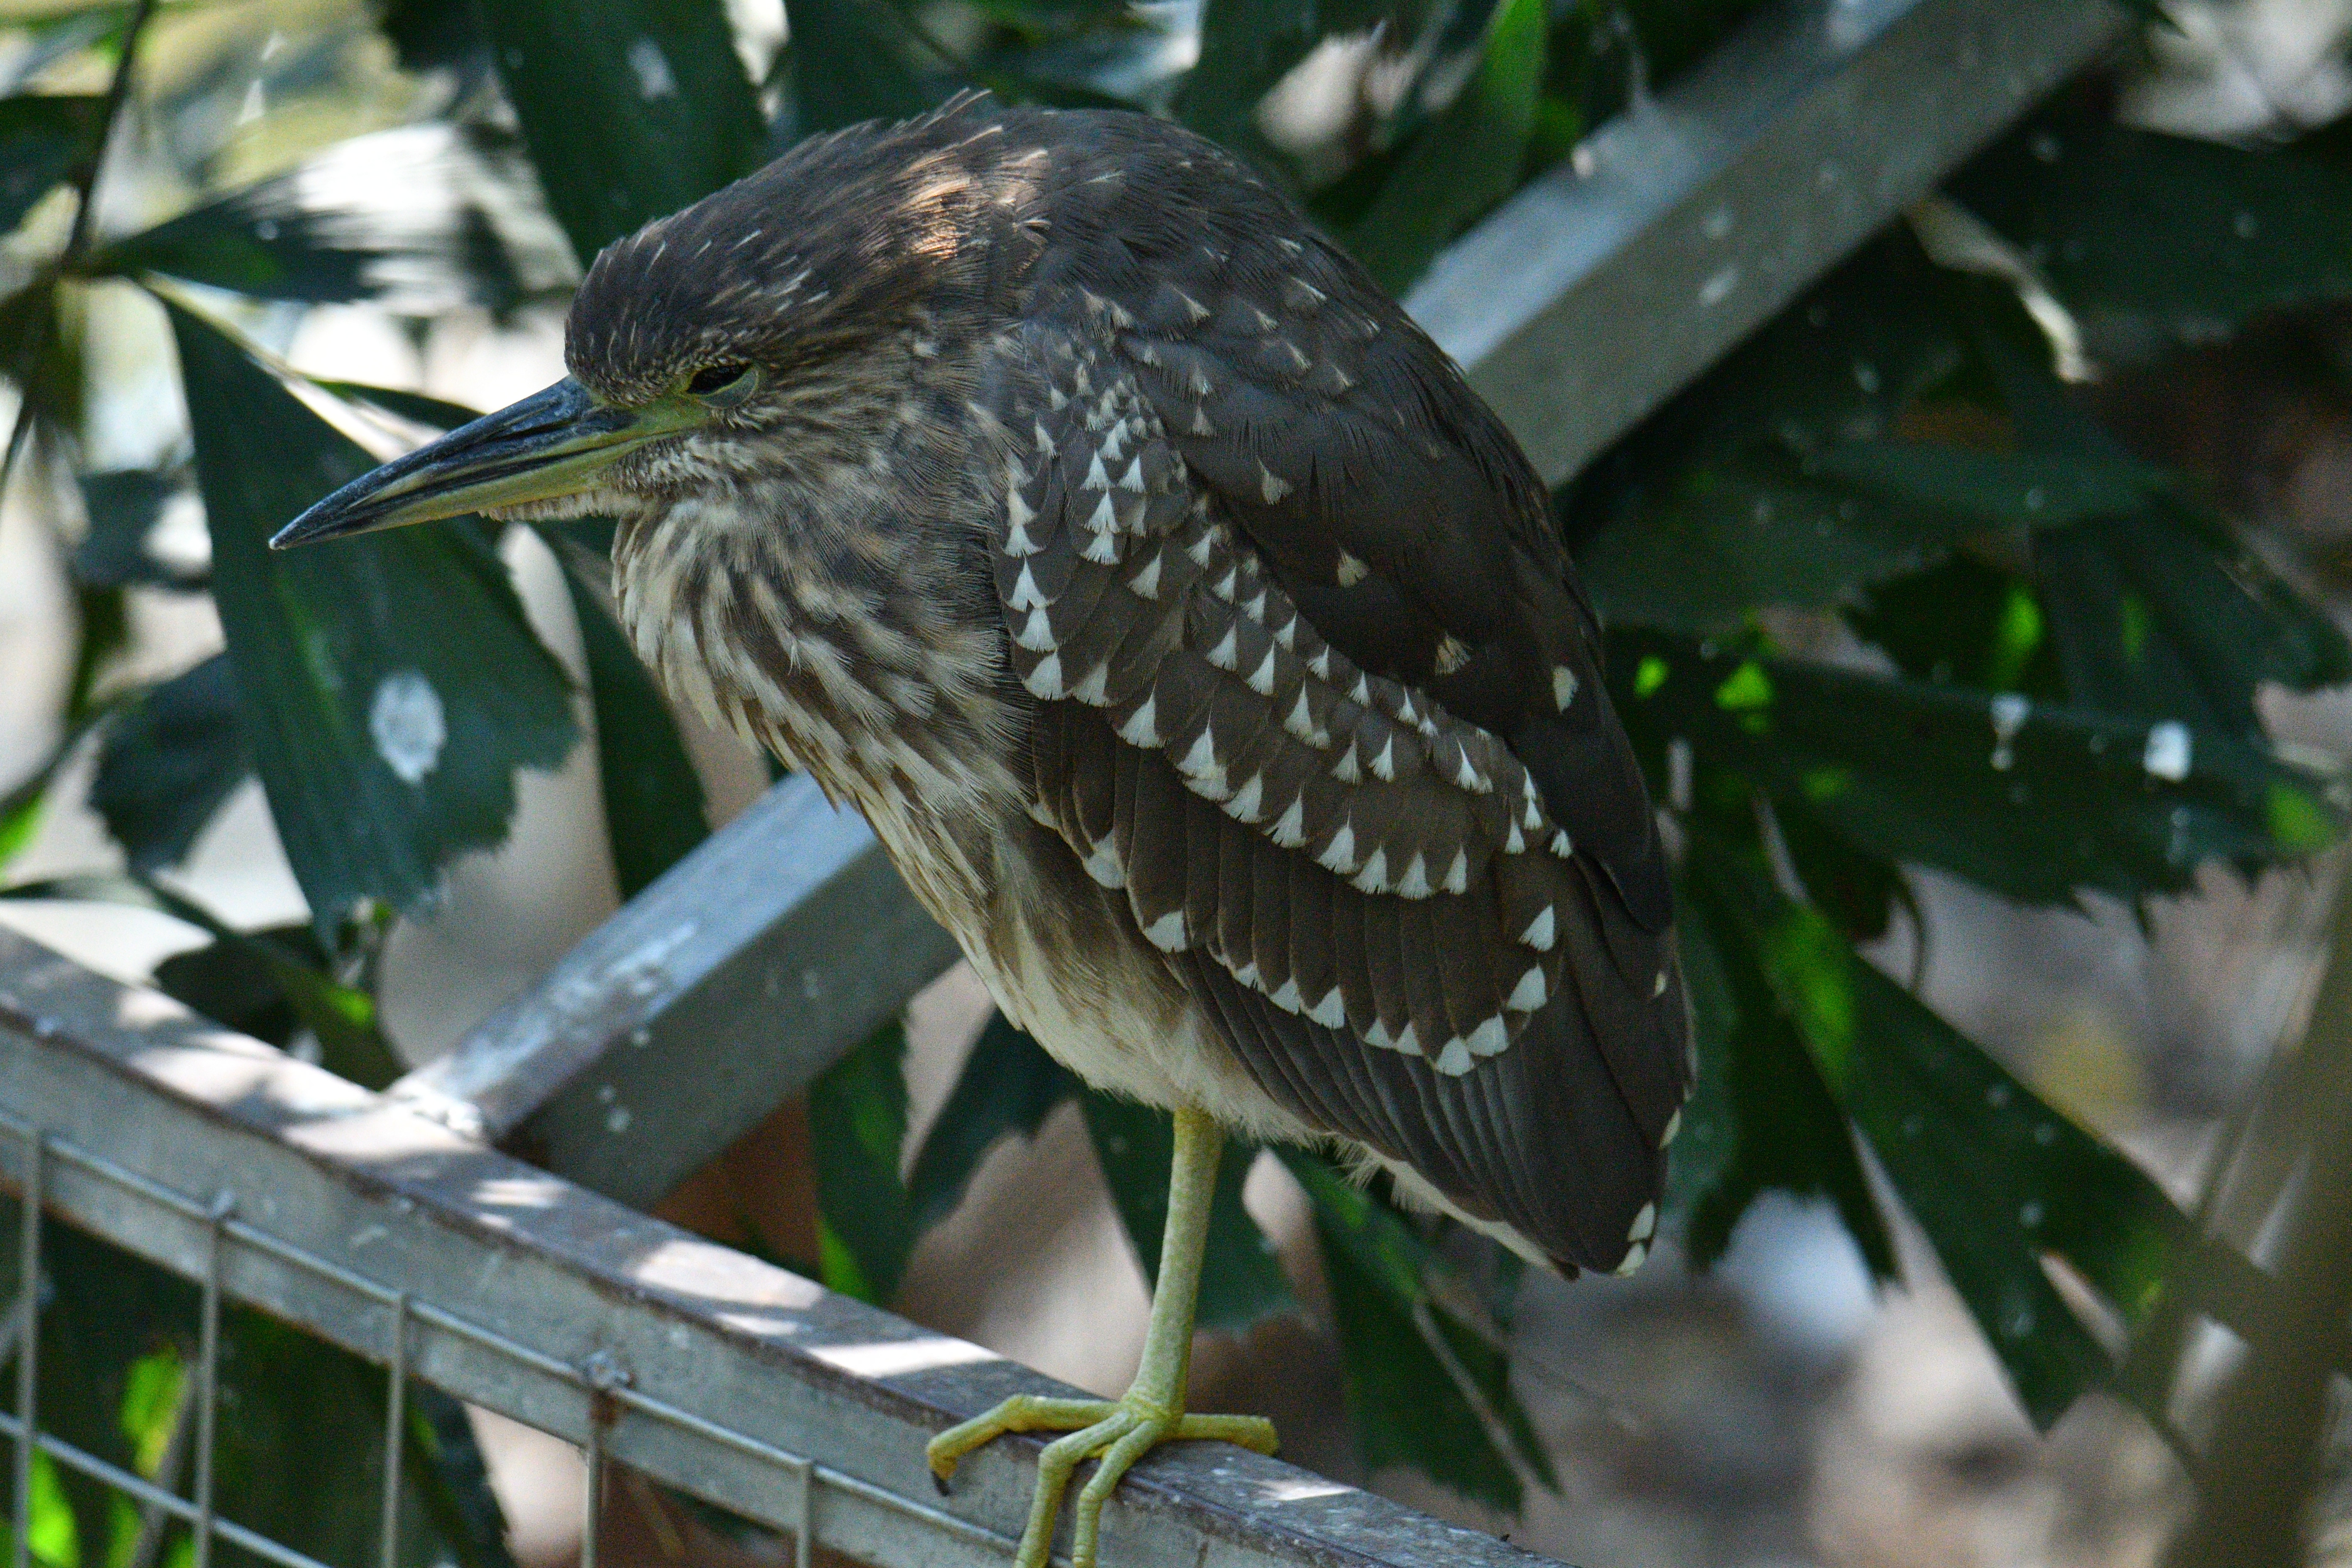
\includegraphics[width=0.3\linewidth]{DSC_4263}
   }
   \subfigure[成年体夜鹭]{
       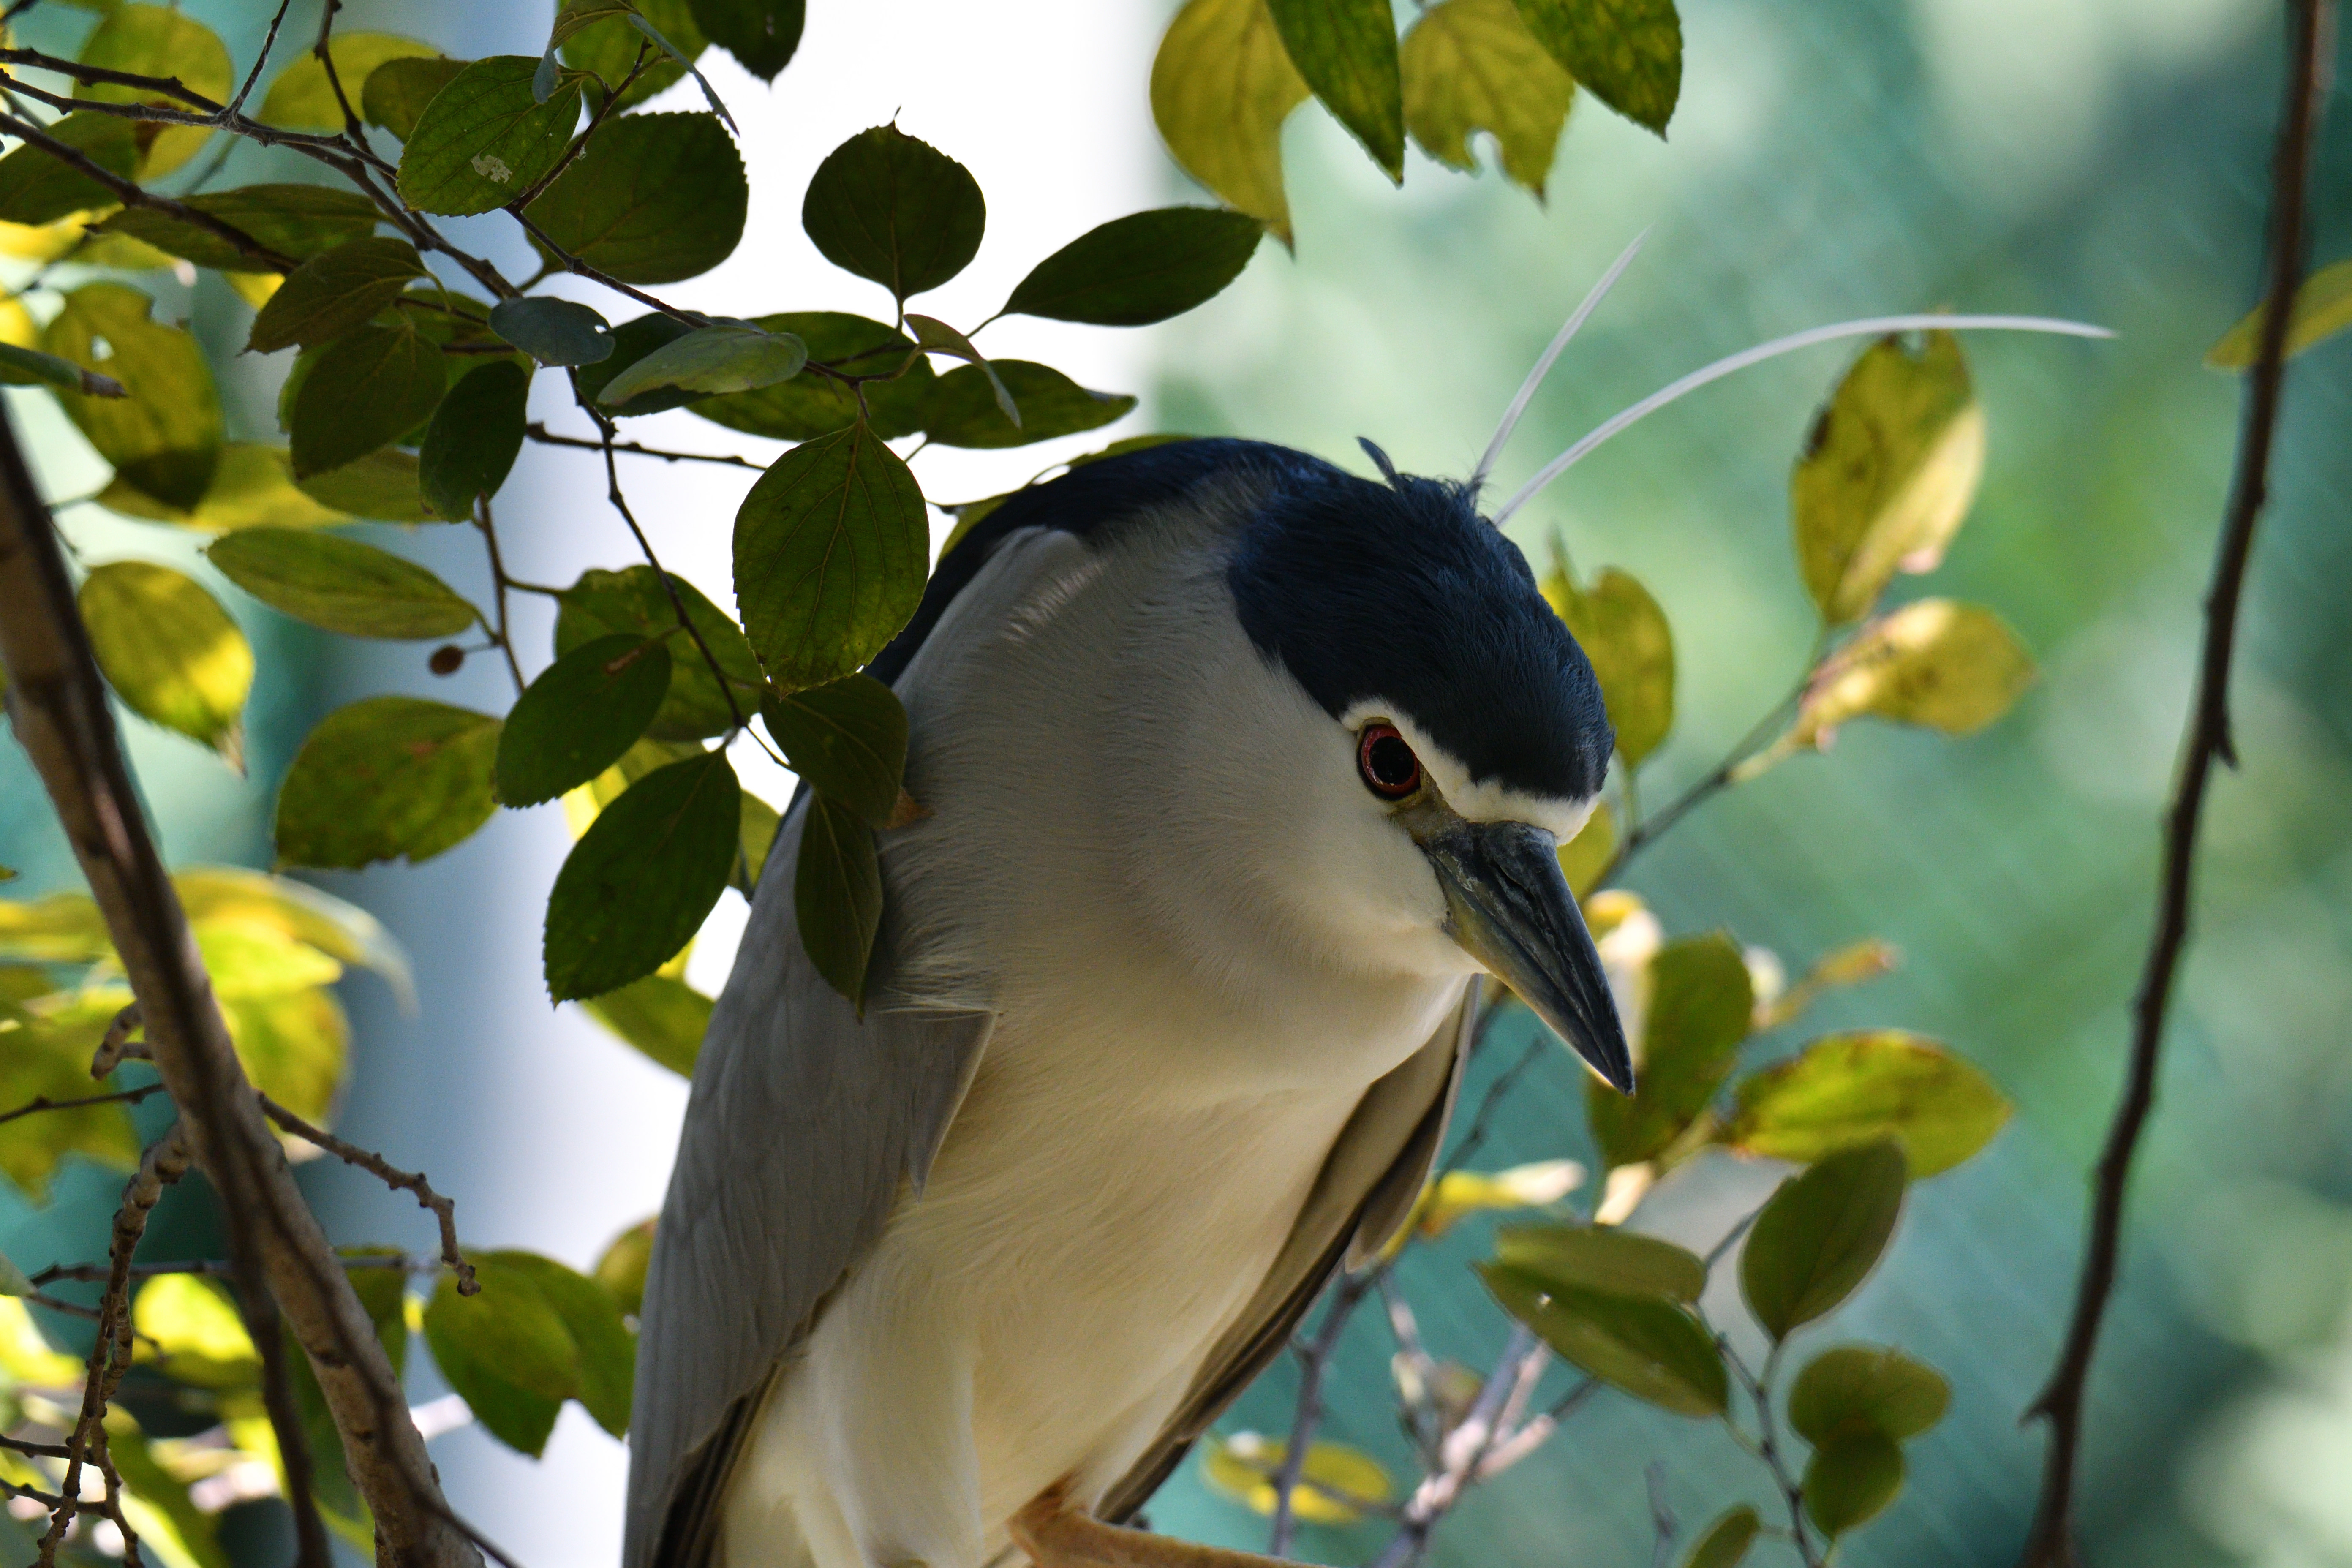
\includegraphics[width=0.3\linewidth]{DSC_4290}
   }
   \subfigure[池鹭]{
       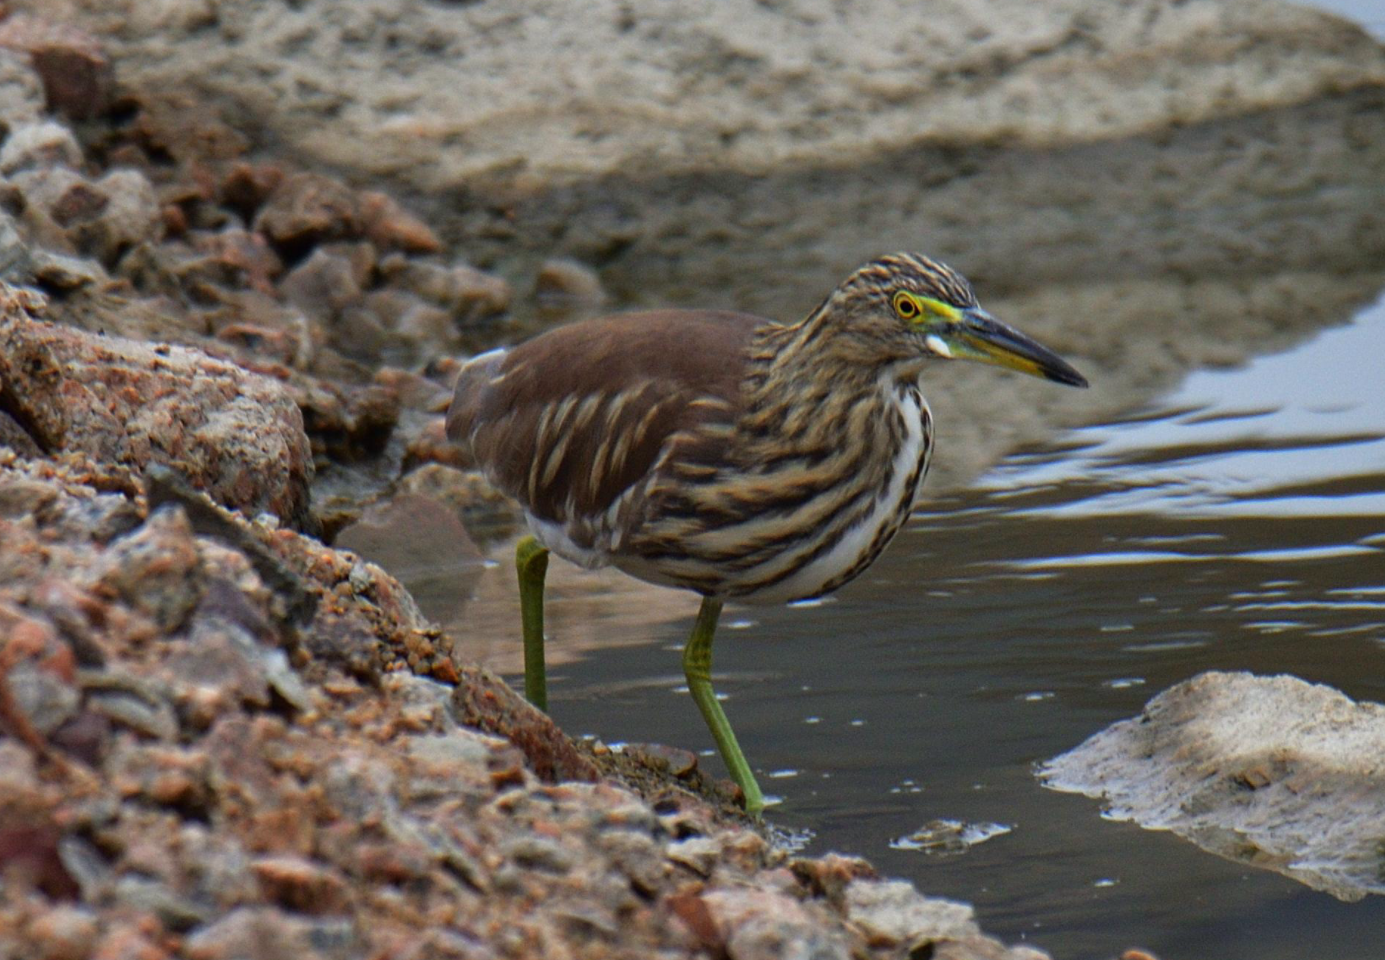
\includegraphics[width=0.3\linewidth]{img1}
   }
   \caption{类内差异大，类间差异小}
\end{figure}



3. 关键区域微小。区分鸟类子类间差异微小，YOLO系列模型缺乏局部判别部件建模能力，
难以胜任这类细粒度任务。\cite{ref4}

4. 鸟类数据规模不足。细粒度识别需要大量的标注数据，但鸟类数据集通常较小，比如著名的CUB-200-2011数据集，每种鸟类只有60张图片。
难以支撑深度模型的训练。\cite{ref4}




\section{模型设计}

\subsection{基本模型 YOLOv8s}

本次选用  YOLOv8s 模型作为基本模型来改进网络，其最大的优势在于平衡了检测精度和部署的复杂度。


\begin{table}[h!]
\centering
\caption{YOLOv8 系列模型性能对比\cite{ref8}}
\label{tab:yolov8_comparison}
\begin{tabular}{lccc}
\hline
模型 & 参数量  & FLOPs & COCO mAP-50  \\
\hline
YOLOv8n & 3.2M & 8.7B & 37.3\%  \\
YOLOv8s & 11.2M & 28.6B & 44.9\%  \\
YOLOv8m & 25.9M & 78.9B & 50.2\%  \\
\hline
\end{tabular}
\end{table}

从表1中可以看到，YOLOv8s在提升了3.5倍左右参数量的情况下，计算能力和推理准确度都相较于 YOLOv8n 模型有明显的提升。
同时，YOLOv8s 在电脑上能够更加方便地训练。


\subsection{改进模型 YOLOv8s-Birds }
\begin{figure}[htbp]
   \centering
   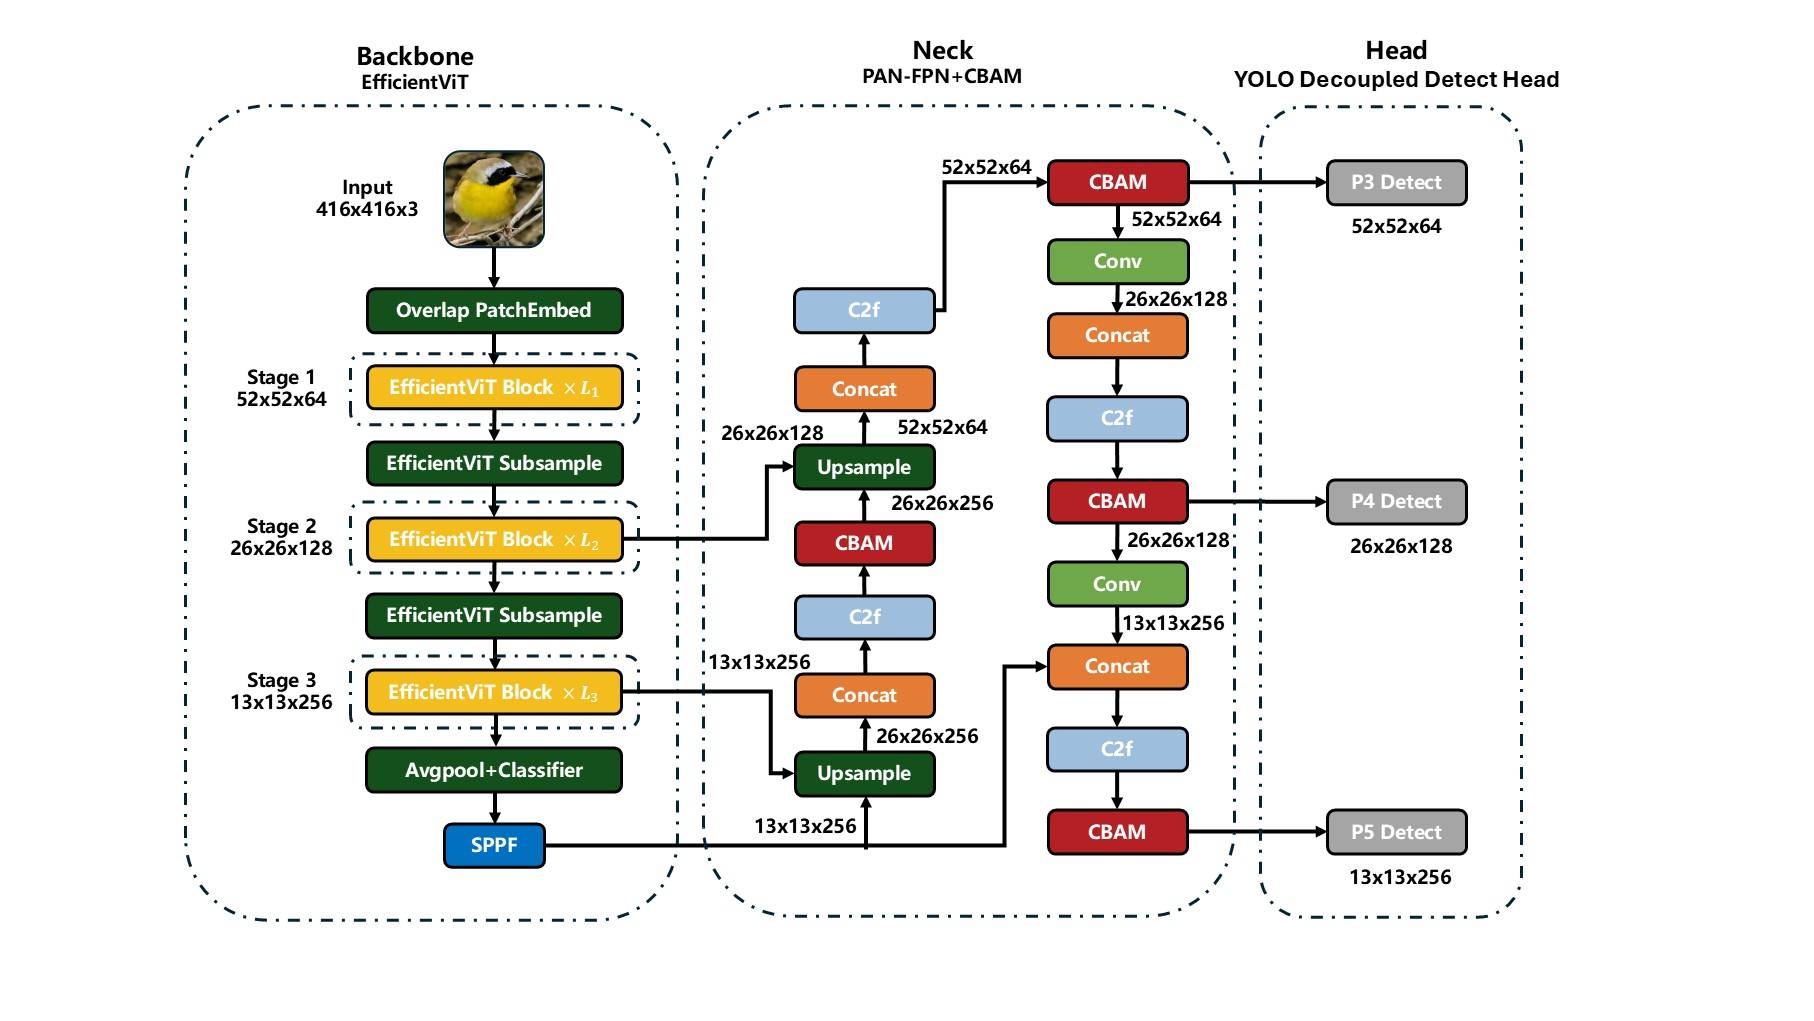
\includegraphics[width=\textwidth]{YOLOv8s-Birds}
   \caption{YOLOv8s-Birds 结构图}
   \label{fig:sample}
\end{figure}

本网络按照原始的YOLOv8系列网络，由 Backbone-Neck-Head 三层结构组成。其中 Backbone 负责特征的提取， Neck 负责特征融合 ，Head 负责最终的检测与分类，如图2。
通过 EfficientViT 网络全局建模，CBAM注意力机制聚焦局部，PAN-FPN金字塔网络多尺度融合信息，该模型在保证轻量化的同时，可以显著地提升对细粒度鸟类的检测于分类能力。

\subsubsection{Backbone: EfficientViT-B1}
YOLOv8s-Birds 使用基于 MIT Han Lab 的 EfficientViT-B1 \cite{ref6} 网络，并为适配检测任务修改 stride ， 从而替换原有的 CSPDarknet 网络。
其核心优势在于可以通过 Lite-MLA 在低计算开销下实现全局上下文建模，可以构建鸟类姿态变化下地非局部部件关联，从而提升识别的准确率。

\begin{table}[h!]
  \begin{center}
    \caption{EfficientVit设置}
    \begin{tabular}{|c c c c|} 
      \hline
      输出 & 尺寸 & stride & 作用 \\
      \hline
      P3 & 52x52x64 & 8 & 获取高分辨率细节 \\

      P4 & 26x26x128 & 2 & 获取中层语义信息\\

      P5 & 13x13x256 & 2 & 获得深层抽象信息 \\
      \hline
    \end{tabular}
  \end{center}
\end{table}

\subsubsection{Neck: PAN-FPN+CBAM}
原有的 YOLOv8 系列使用了 PAN-FPN 金字塔架构，其目的在于充分利用 Backbone 中得到的多尺度特征。
而 YOLOv8s-Birds 在此基础上，在每级融合后插入 CBAM\cite{ref7} 注意力机制，之后再交给检测头进行识别和分类的任务，使模型可以聚焦于局部特征，从而提升识别的准确率。 

\subsubsection{Head:YOLO Decoupled Detect Head}
YOLOv8s-Birds 延用了 YOLOv8 系列中三个解耦式检测头的设计，其分别具有不同的作用。

\begin{table}[h!]
  \begin{center}
    \caption{三个检测头的作用}
    \begin{tabular}{|c c c|} 
      \hline
      检测头 & 输入大小 & 作用 \\
      \hline
      P5 Detect & 52x52x64 &  整体姿态\\

      P4 Detect & 26x26x128 & 中距离目标\\

      P3 Detect & 13x13x256 & 局部信息 \\
      \hline
    \end{tabular}
  \end{center}
\end{table}


\section{改进思路与理论依据}

\subsection{分析现有模型的问题}
根据 1.2 节中的分析，我们的网络旨在解决以下两个个主要的问题：

1. YOLOv8 backbone使用的 CSPDarknet 网络结构依赖堆叠卷积扩大感受野，但其局部的长距离关联建模能力弱。


2. YOLOv8 neck 使用的 PAN-FPN 的特征拼接操作平等对待所有通道与空间位置，无法显式强化关键局部区域，易受复杂背景干扰。


3. 尺度变化剧烈：图像中鸟类可能占据从几十像素到数百像素不等的空间范围。


所以，针对以上的两个痛点，引入了 EfficientViT 、 CBAM 和对比学习机制进行优化。


\subsection{引入 EfficientViT 网络}

\subsubsection{现有问题}
YOLOv8 Backbone 中原有的 CSPDarknet 网络属于传统的 CNN ，其通过层级卷积逐步聚合局部信息，但是其感受野增长缓慢，
难以实现长距离建模依赖。而鸟类识别通常需要跨区域的语义关联。

同时， ViT(Vision Transformer) 通过自注意力机制本身支持全局交互，但是标准的 ViT 计算复杂度高达
$O(n^2)$ ，难以实现移动端实时设备的部署任务\cite{ref9}。

\subsubsection{EfficientViT 理论依据}  
\begin{figure}[htbp]
   \centering
   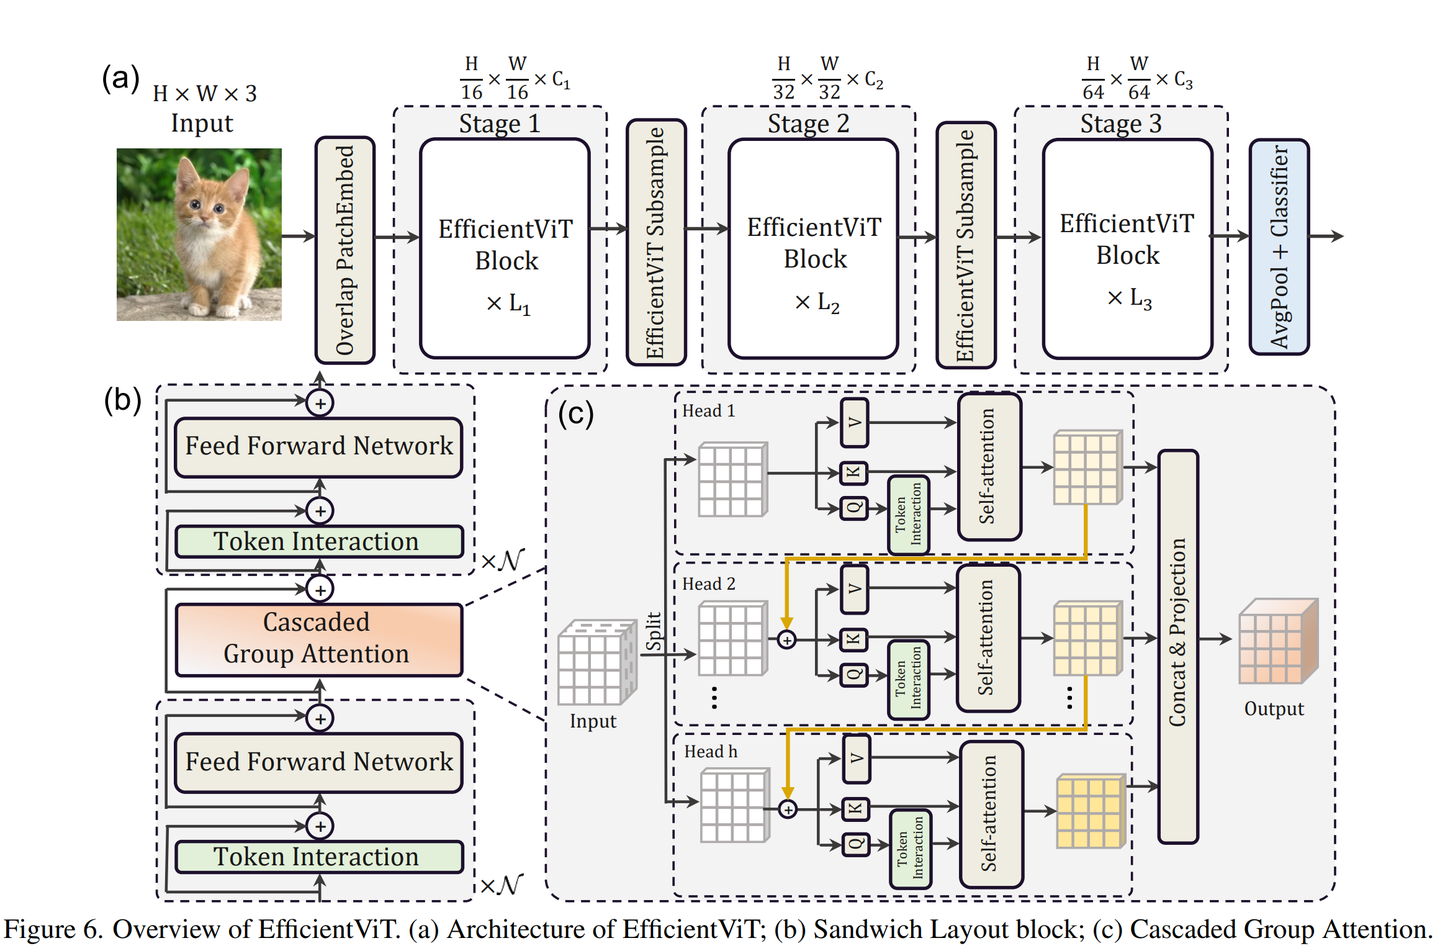
\includegraphics[width=0.8\textwidth]{EfficientViT}
   \caption{EfficientViT 网络\cite{ref6}}
\end{figure}

EfficientViT \cite{ref6} 是一种高效的视觉 transformer 模型，它是基于 ViT 网络的一种改进网络。前者相较于后者建模能力更强，并且计算开销更小，推理速度更快，更适合本任务部署在移动设备端的要求。它通过一种新设计的“三明治”架构块
和引入级联分组注意力机制，如图3，减少了计算的冗余与模型的性能。EfficientViT 采用典型的金字塔结构，主干部分使用 stride=2 的卷积快速下采样。其包含的多个 stage 中每个 stage 都包含若干 EfficientViT Blocks，逐步下采样，通道数递增.
同时还采取了全局平均池化+全连接层的轻量分类头。

针对这个鸟类识别任务，采用 MIT Han Lab 的 EfficientViT-B1网络\cite{ref10}，并且对 stride 进行了更独特的优化，其具体参数见 2.2.1 节。

EfficientViT-B1 模块的核心实现的源码见附件A。




\subsection{引入CBAM注意力机制}

\subsubsection{现有问题}
在鸟类识别任务中，通常面临鸟内目标很小，或者需要分辨的特征部位很小的问题。
原有的 PAN-FPN 金字塔网络的特征融合能力虽然可以融合多尺度信息，但是其内部没有原生的注意力机制，
无法锁定关注一些重要特征。在原本的网络中引入注意力机制，可以抑制大面积的背景信息，让网络集中于关键的局部信号。

\subsubsection{CBAM 理论依据}

CBAM（Convolutional Block Attention Module）\cite{ref7} 是一种轻量级双重注意力机制。
它的结构如图3所示。CBAM对于输入的图像，先进行通道注意力的加权，再进行空间注意力的处理。

\begin{figure}[htbp]
   \centering
   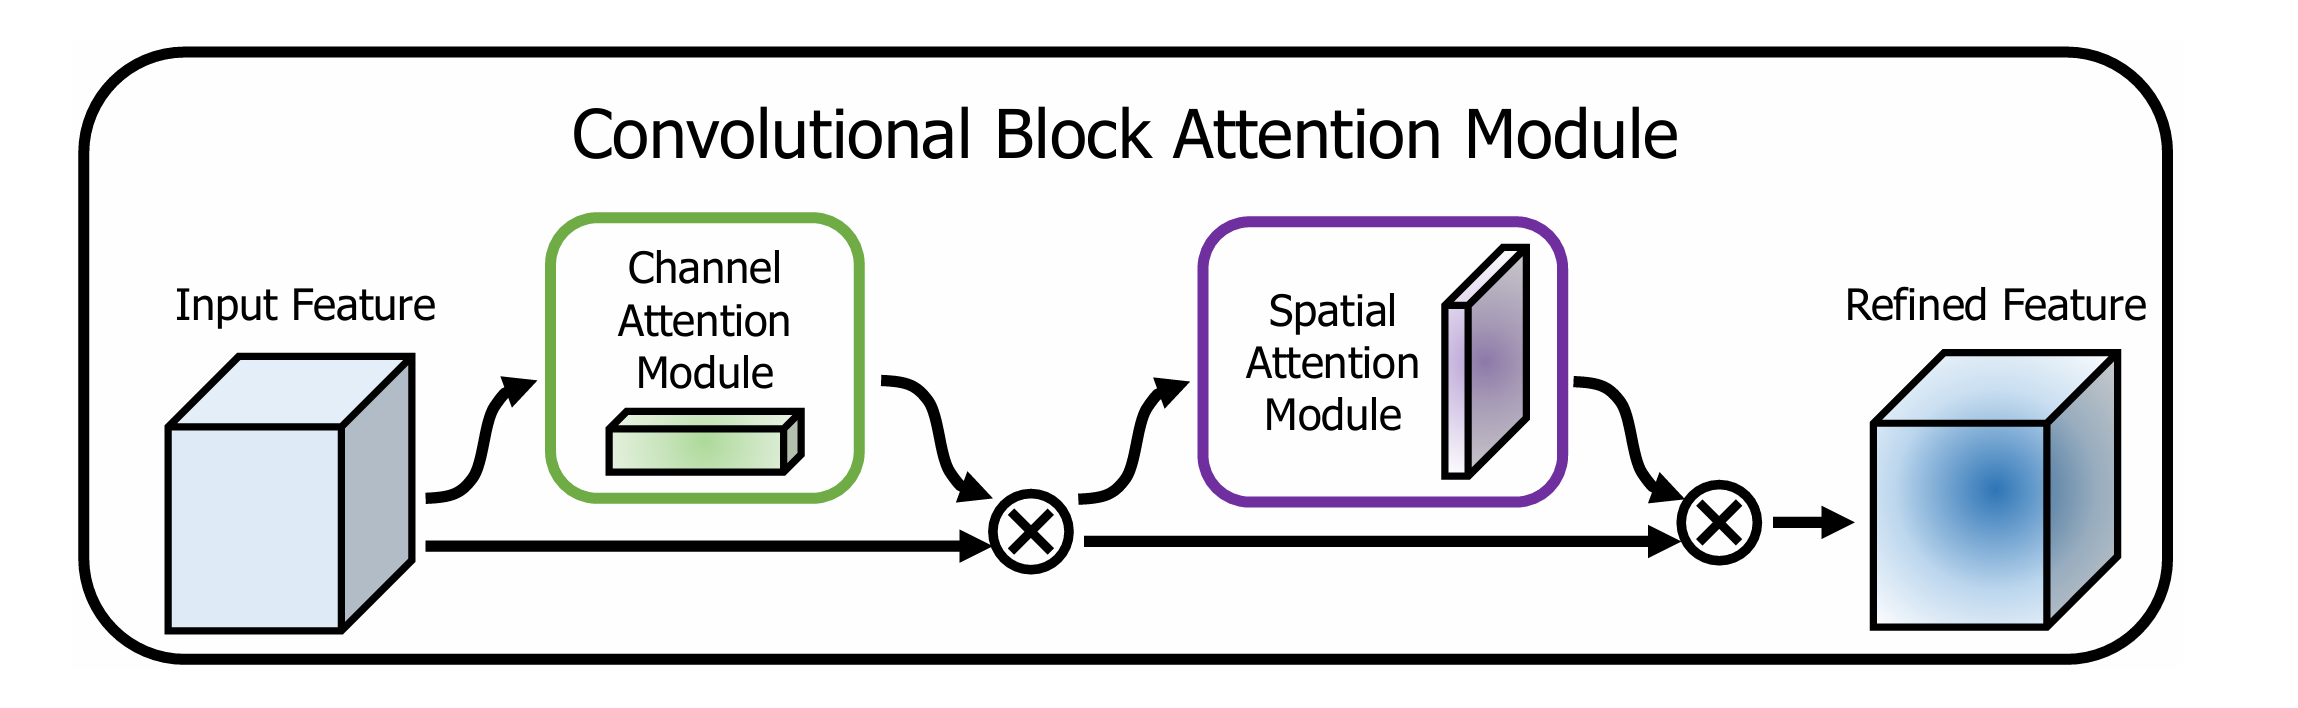
\includegraphics[width=\textwidth]{CBAM-overall}
   \caption{CBAM注意力机制\cite{ref7}}
\end{figure}


其主要由两部分组成：

1. 通道注意力机制。通道注意力主要通过全局平均池化和全局最大池化，将输出的结果送进共享全连接层，
对两个结果做加法并且归一化，通过建模不通特征通道的相关性，获取到每个通道的重要程度并赋予不同的权重系数，
从而强化重要的特征同时抑制非重要的特征。

2. 空间注意力机制。空间注意力机制在输入图像的每一个特征点的通道上取最大值和平均值，之后对这两个结果进行拼接、压缩和归一化。
得到每个位置上的权重，从而加强对特定区域的关注而减少对不相关区域的关注。

\begin{figure}[htbp]
   \centering
   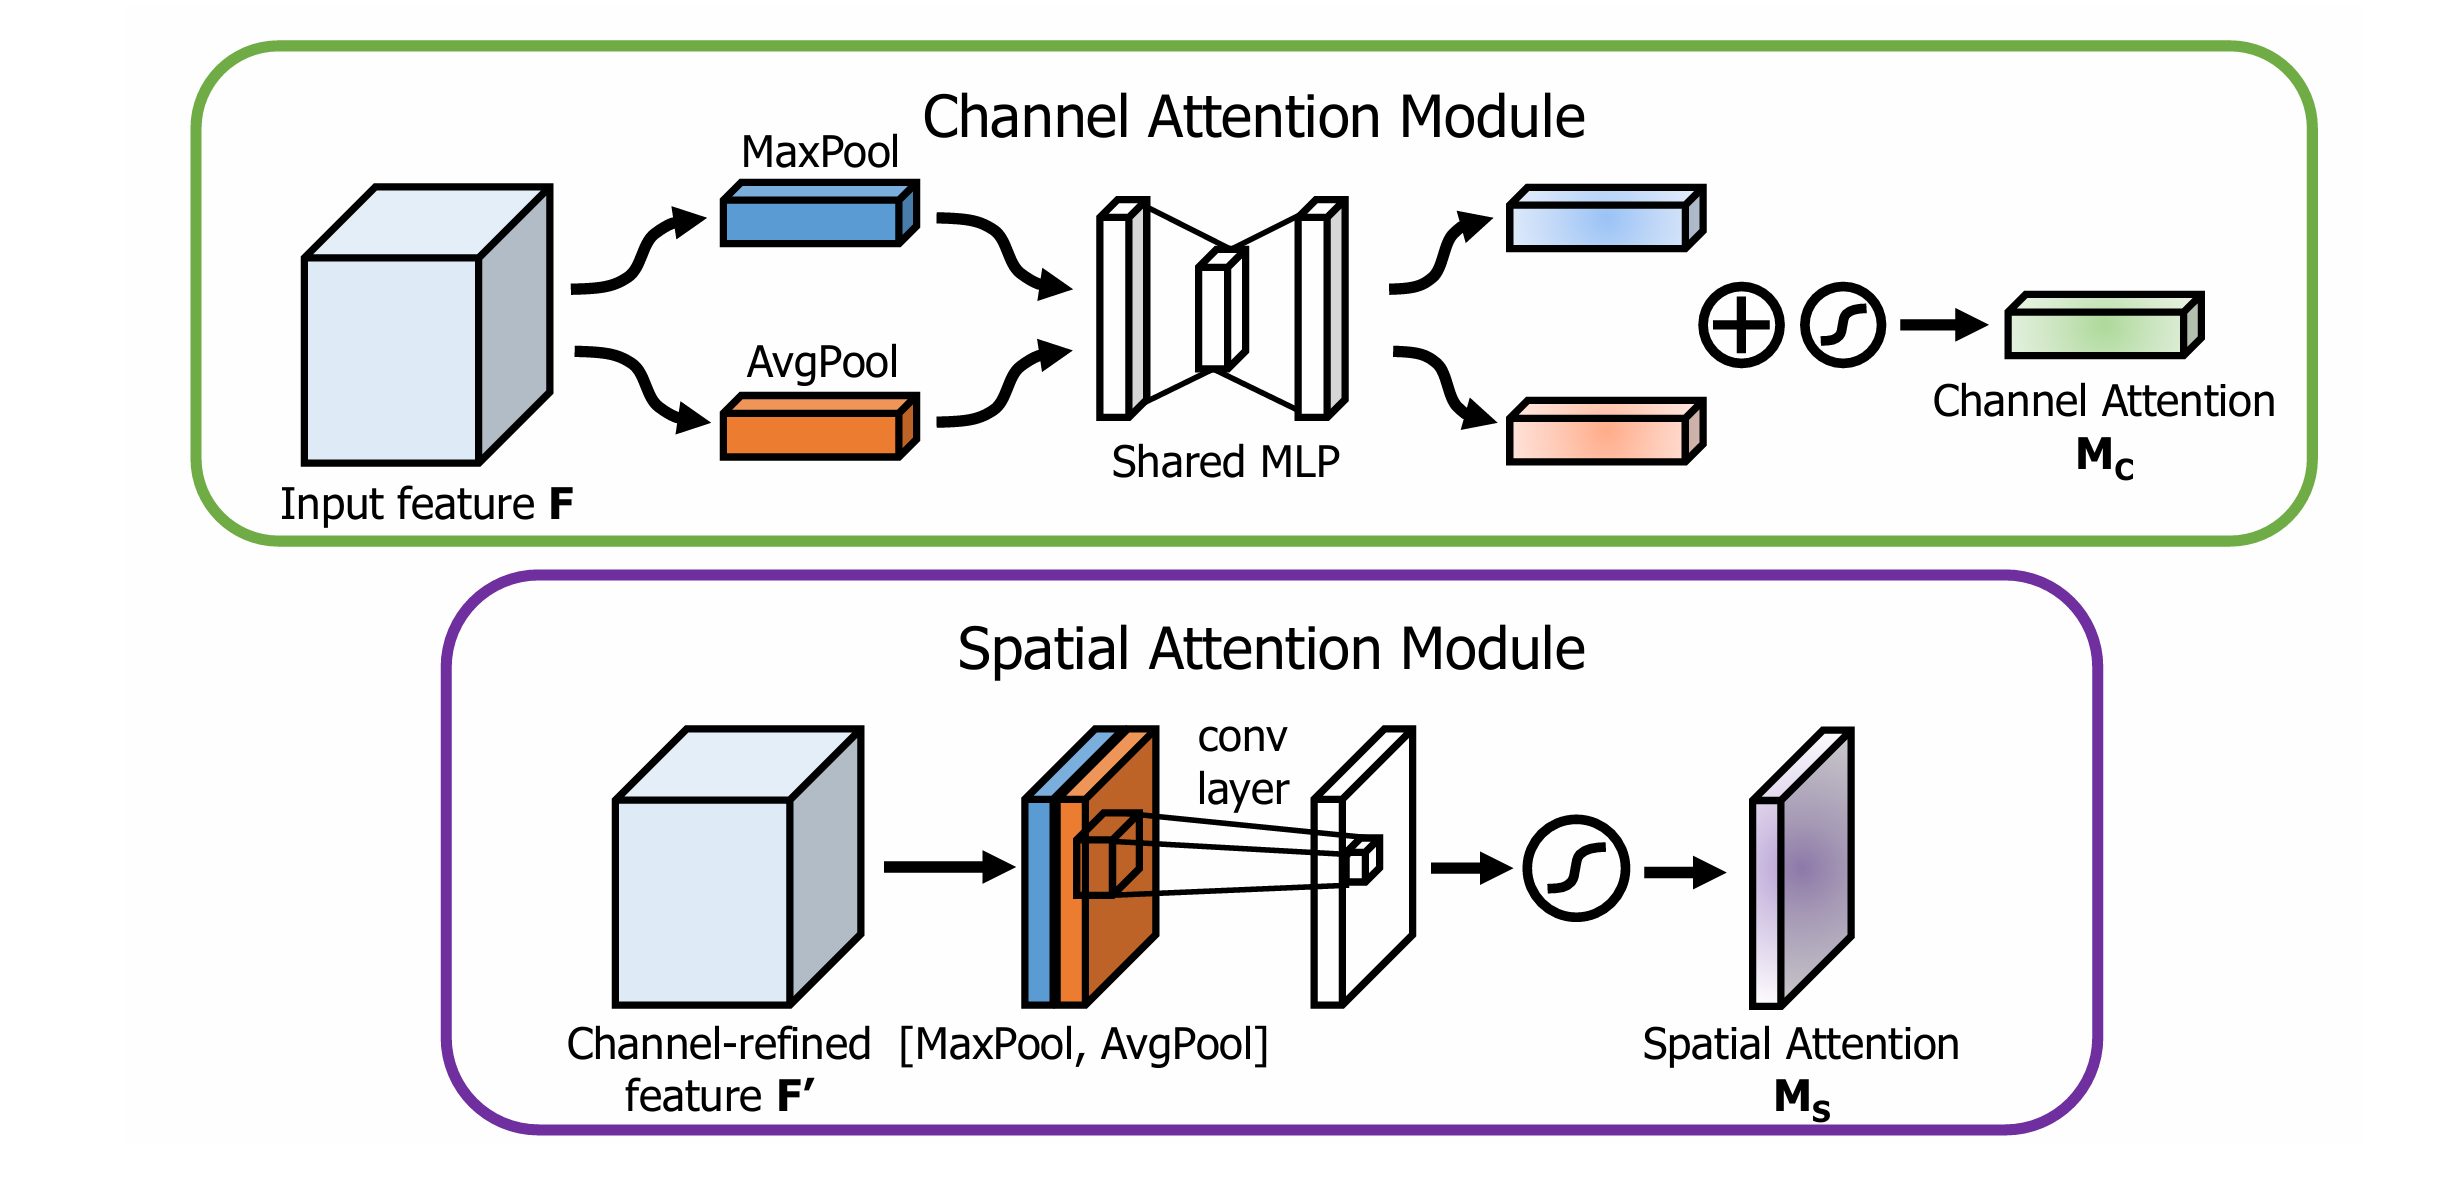
\includegraphics[width=\textwidth]{CBAM-sp}
   \caption{CBAM注意力机制中的通道注意力和空间注意力\cite{ref7}}
\end{figure}

CBAM模块的核心实现的源码见附件B。


\subsection{引入对比学习预训练策略}

\subsubsection{现有问题}

现有的 CUB-200 数据集样本太小，且标注鸟类数据集所需要的专业知识成本巨高，可以使用类似 iNaturalist\cite{ref11} 这种无标签的海量无标注数据进行辅助学习。

\subsubsection{对比学习理论策略}
为进一步提升模型的判别能力，我们期望将在预训练阶段引入对比学习。
我们使用 SimCLR 框架在 CUB-200 训练集上对 EfficientViT backbone 进行自监督预训练\cite{ref12}，
通过拉近同一图像不同增强视图的特征表示、推开不同图像的表示，使模型学习到对姿态、光照变化鲁棒的鸟类表征。
该策略无需额外的人工标注，且可以完美融合进现有检测架构，可以缓解小样本过拟合的问题。

并且我们将采用两阶段训练策略：
阶段一（无监督预训练）：

1. 使用 iNaturalist 2021 鸟类子集；

2. 以 EfficientViT-B1 为编码器，采用 SimCLR 框架进行对比学习；

3. 数据增强：随机裁剪、色彩抖动、高斯模糊。

阶段二（有监督微调）：

1. 冻结 backbone 前两层，微调其余部分 + Neck + Head；

2. 在 CUB-200 上端到端训练。


\section{实验方案}

\subsection{数据集的准备}
本次实验采用CUB-200-2011（Caltech-UCSD Birds-200-2011）细粒度视觉分类数据集，该数据集包含北美常见的200种鸟类，
每种鸟类大约60张图像，共11,788张图像，每张图片均提供了类别标签和人工标注的粗略边界框。\cite{ref4}

为构建适配YOLOv8s模型训练的数据，我们对原始数据进行了如下预处理：

1. 目录结构重组：将图像按官方划分的训练验证数据集大小$1:1$分别存入 images/train 与 images/val 目录，一共得到训练集5,994张，测试集5,794张。

2. 标签格式转换：将原始以像素为单位的边界框坐标归一化为 YOLO 格式，并保存为与图片名字一一对应 .txt 文件。

3. 类别映射对齐：确保 cub.yaml 配置文件中的 names 字段严格遵循 CUB 官方类别顺序。

4. 训练数据增强：所有的训练图像在训练过程中统一被压缩为416x416分辨率，并应用Mosaic、Copy-paste、色调扰动、明度扰动、饱和度扰动等数据增强策略以提升模型的泛化能力。

\subsection{实验设计与评价指标}

本实验将采用对比实验，将未改进的 YOLOv8s模型 与 改进后的 YOLOv8s-Birds 模型 在 CUB-200-2011数据集上进行训练。



并且将从以下三个指标来评估模型的能力：

1. 精确率(Precision)：表示预测为正类的样本中有多少是真正类。即所有被模型预测为鸟的部分中，实际是鸟的比例。

$$
Precision = \frac{TP}{TP+FP}
$$

2. 召回率(Recall)：表示真实为正类的样本中有多少被正确预测为正类。即所有真实的鸟中，被模型正确检测出来的比例。

$$
Recall = \frac{TP}{TP+FN}
$$

3. 平均精度均值（mAP, Mean Average Precision）：用于计算了不同IoU（Intersection over Union，交并比）阈值下AP（每个类别的平均精度）的平均值。
有 mAP50 和 mAP50-95 两个细分指标。

两个模型的训练都在同一台电脑上进行，并且采用相同的配置参数进行训练（见表1）。

\begin{table}[h!]
  \begin{center}
    \caption{训练参数设置表}
    \begin{tabular}{|c|c|c|} 
      \hline
      参数 & 含义 & 设置 \\
      \hline
      model & 训练模型 & yolov8s.yaml / yolov8s-Birds.yaml \\
      \hline
      data & 数据集配置文件 & cub.yaml  \\
      \hline
      epoches & 训练轮数 & 100 \\
      \hline
      patience & 若多少轮mAP不升则停止 & 15 \\
      \hline
      batch & 批量处理大小 & 8 \\
      \hline
      mosaic & mosaic数据增强算法 & 1.0  \\
      \hline
      workers & 工作线程数 & 0 \\
      \hline
      copy\_paste & copy\_paste数据增强 & 0.3  \\
      \hline
      close\_mosaic & 最后多少轮关闭mosaic & 10 \\
      \hline
      hsv\_h & 色调扰动 & 0.015 \\
      \hline
      hsv\_s & 饱和度扰动 & 0.7 \\
      \hline
      hsv\_v & 明度扰动 & 0.4 \\
      \hline
    \end{tabular}
  \end{center}
\end{table}

\subsection{实验结果与数据分析}

\begin{table}[h!]
  \begin{center}
    \caption{实验结果}
    \begin{tabular}{|c|c|c|c|c|} 
      \hline
      模型 & 精确率(Precision) & 召回率(Recall) & mAP50 & mAP50-95 \\
      \hline
      YOLOv8s & 75\% & 73\% & 78\% & 69\% \\
      \hline
      YOLOv8s-Birds(预期) & 78\% - 81\% & 78\% - 82\% & 83\% - 86\% & 74\% - 78\% \\
      \hline
    \end{tabular}
  \end{center}
\end{table}

\newpage
如表5所示，本模型在 CUB-200 测试集上实现了全面性能提升。
与基本的 YOLOv8s 相比，
精确率提升至 78\%～81\%，验证了 CBAM 注意力机制在抑制背景干扰方面的有效性。
召回率从 73\% 提升至 78\%～82\%，表明改进后的网络显著增强了对小尺度、局部判别性特征（如喙形、眼斑）的检出能力。
mAP50 从 78\% 提升至 83\% - 86\%，反映出模型整体检测精度的显著提高。
同时，mAP50-95 从 69\% 提升至 74\%～78\%，说明高 IoU 下的定位鲁棒性得到强化。
综合来看，本文提出的 YOLOv8s-Birds 框架在精度、召回与定位稳定性上均优于原始模型。


\section{结论与未来展望}
\subsection{结论}

本文针对细粒度鸟类目标检测任务中小目标漏检严重、背景干扰强、类内差异大等核心挑战，提出了一种轻量高效的检测架构。该模型以 YOLOv8 为基础框架，并在此基础上提出三项关键改进：

1. 将主干网络替换为具备全局建模能力的 EfficientViT-B1。

2. 在特征金字塔网络中嵌入 CBAM 通道-空间双重注意力机制。

3. 探索对比学习预训练策略 以增强特征判别性。

以上三项改进后的网络在精确率、召回率、mAP50和mAP50-95 总体水平相较于原始模型有很大的提升。

\subsection{局限性分析}
尽管改进模型总体上已经取得了显著提升，但仍存在若干局限性：
\begin{itemize}
  \item 对数据依赖性强：对比学习预训练的效果高度依赖于额外数据源的质量与规模，鸟类数据集具有天生规模小质量差的的特点。
  \item 计算开销略大：EfficientViT 虽比标准 ViT 轻量，但仍比 CSPDarknet 多约 15\% FLOPs，部署在部分小型低功耗设备上具有一定的挑战。
  \item 类别不平衡未显式处理：CUB-200 中部分稀有鸟种样本极少，模型对其检测性能仍不理想，现有损失函数未针对性优化长尾分布问题。
\end{itemize}

\subsection{未来改进方向}

针对未来关于鸟类识别的方向，可以从以下几个方向进行改进：

\begin{itemize}
  \item 更高效的 ViT 架构设计。探究更高效的 ViT 机制以便于该模型在更轻量化更低能耗的设备上部署。
  \item 细粒度专用注意力机制。根据鸟类的生物学特征，设计专门的细粒度注意力机制提升识别的准确率。
  \item 多模态融合扩展。针对野外鸟类识别的具体场景，融合音频信息与视觉信息，构建跨模态检测系统。
\end{itemize}




\newpage
\begin{thebibliography}{99}  

\bibitem{ref1} 张利民,杨君子,代孟杰,等. 基于改进YOLOv8的衡水湖湿地鸟类识别研究 [J]. 衡水学院学报, 2025, 27 (04): 1-8.

\bibitem{ref2} 李茂晖,吴传平,鲍艳,等. 论YOLO算法在机器视觉中应用原理 [J]. 教育现代化, 2018, 5 (41): 174-176. DOI:10.16541/j.cnki.2095-8420.2018.41.077.

\bibitem{ref3} 韩涛. 基于YOLOv8的鸟类目标检测与识别方法研究[D]. 大连交通大学, 2025. DOI:10.26990/d.cnki.gsltc.2025.001020.

\bibitem{ref4} Wah C, Hornbrook B, Branson K, et al. The Caltech-UCSD Birds-200-2011 Dataset[R]. California Institute of Technology, 2011.

\bibitem{ref5} Liu, S., et al. (2022). "Small Object Detection in Remote Sensing Images: A Survey." IEEE Journal of Selected Topics in Applied Earth Observations and Remote Sensing, 15, 7498–7516.

\bibitem{ref6} CAI H, GAN C, HAN S. EfficientViT: Memory efficient vision transformer with cascaded group attention[C]// International Conference on Learning Representations. 2023.

\bibitem{ref7} WOO S, PARK J, LEE J Y, et al. CBAM: Convolutional block attention module[C]// Proceedings of the European Conference on Computer Vision (ECCV). 2018: 3–19.

\bibitem{ref8} G. Jocher, A. Chaurasia, and J. Qiu, Ultralytics YOLOv8, version 8.0.0. GitHub, 2023. [Online]. Available: https://github.com/ultralytics/ultralytics 

\bibitem{ref9} Dosovitskiy, A., Beyer, L., Kolesnikov, A., Weissenborn, D., Zhai, X., Unterthiner, T., ...  Houlsby, N. (2020). An Image is Worth 16x16 Words: Transformers for Image Recognition at Scale. In Proceedings of the International Conference on Learning Representations (ICLR).

\bibitem{ref10} H. Cai, J. Li, M. Hu, C. Gan, and S. Han, "EfficientViT: Lightweight Multi-Scale Attention for High-Resolution Dense Prediction," in Proc. IEEE/CVF Int. Conf. Comput. Vis. (ICCV), 2023, pp. 17302–17313.

\bibitem{ref11} HORN G V, MAC AODHA O, et al. The iNaturalist Species Classification and Detection Dataset 2021[EB/OL]. (2021-05-20) [2026-01-17]. https://arxiv.org/abs/2105.09864.

\bibitem{ref12} CHEN T, KORNBLITH S, NOROUZI M, et al. A Simple Framework for Contrastive Learning of Visual Representations[EB/OL]. (2020-06-15) [2026-01-17]. https://arxiv.org/abs/2002.05709.

\end{thebibliography}

\appendix
\section{EfficientViT 主干网络}
\lstset{language=python}
\begin{lstlisting}
import torch
import torch.nn as nn
import torch.nn.functional as F
import torch.utils.checkpoint as checkpoint
import itertools
 
from timm.models.layers import SqueezeExcite
 
import numpy as np
import itertools
 
__all__ = ['EfficientViT_M0', 'EfficientViT_M1', 'EfficientViT_M2', 
'EfficientViT_M3', 'EfficientViT_M4', 'EfficientViT_M5']
 
class Conv2d_BN(torch.nn.Sequential):
    def __init__(self, a, b, ks=1, stride=1, pad=0, dilation=1,
                 groups=1, bn_weight_init=1, resolution=-10000):
        super().__init__()
        self.add_module('c', torch.nn.Conv2d(
            a, b, ks, stride, pad, dilation, groups, bias=False))
        self.add_module('bn', torch.nn.BatchNorm2d(b))
        torch.nn.init.constant_(self.bn.weight, bn_weight_init)
        torch.nn.init.constant_(self.bn.bias, 0)
 
    @torch.no_grad()
    def switch_to_deploy(self):
        c, bn = self._modules.values()
        w = bn.weight / (bn.running_var + bn.eps)**0.5
        w = c.weight * w[:, None, None, None]
        b = bn.bias - bn.running_mean * bn.weight / \
            (bn.running_var + bn.eps)**0.5
        m = torch.nn.Conv2d(w.size(1) * self.c.groups, w.size(
            0), w.shape[2:], stride=self.c.stride, padding=self.c.padding, 
            dilation=self.c.dilation, groups=self.c.groups)
        m.weight.data.copy_(w)
        m.bias.data.copy_(b)
        return m
 
def replace_batchnorm(net):
    for child_name, child in net.named_children():
        if hasattr(child, 'fuse'):
            setattr(net, child_name, child.fuse())
        elif isinstance(child, torch.nn.BatchNorm2d):
            setattr(net, child_name, torch.nn.Identity())
        else:
            replace_batchnorm(child)
            
 
class PatchMerging(torch.nn.Module):
    def __init__(self, dim, out_dim, input_resolution):
        super().__init__()
        hid_dim = int(dim * 4)
        self.conv1 = Conv2d_BN(dim, hid_dim, 1, 1, 
        0, resolution=input_resolution)
        self.act = torch.nn.ReLU()
        self.conv2 = Conv2d_BN(hid_dim, hid_dim, 3, 
        2, 1, groups=hid_dim, resolution=input_resolution)
        self.se = SqueezeExcite(hid_dim, .25)
        self.conv3 = Conv2d_BN(hid_dim, out_dim, 1, 1, 
        0, resolution=input_resolution // 2)
 
    def forward(self, x):
        x = self.conv3(self.se(self.act(self.conv2(self.act(self.conv1(x))))))
        return x
 
 
class Residual(torch.nn.Module):
    def __init__(self, m, drop=0.):
        super().__init__()
        self.m = m
        self.drop = drop
 
    def forward(self, x):
        if self.training and self.drop > 0:
            return x + self.m(x) * torch.rand(x.size(0), 1, 1, 1,
            device=x.device).ge_(self.drop).div(1 - self.drop).detach()
        else:
            return x + self.m(x)
 
 
class FFN(torch.nn.Module):
    def __init__(self, ed, h, resolution):
        super().__init__()
        self.pw1 = Conv2d_BN(ed, h, resolution=resolution)
        self.act = torch.nn.ReLU()
        self.pw2 = Conv2d_BN(h, ed, bn_weight_init=0, resolution=resolution)
 
    def forward(self, x):
        x = self.pw2(self.act(self.pw1(x)))
        return x
 
 
class CascadedGroupAttention(torch.nn.Module):
    r""" Cascaded Group Attention.
    Args:
        dim (int): Number of input channels.
        key_dim (int): The dimension for query and key.
        num_heads (int): Number of attention heads.
        attn_ratio (int): 
        Multiplier for the query dim for value dimension.
        resolution (int): 
        Input resolution, correspond to the window size.
        kernels (List[int]): The kernel size of the dw conv on query.
    """
    def __init__(self, dim, key_dim, num_heads=8,
                 attn_ratio=4,
                 resolution=14,
                 kernels=[5, 5, 5, 5],):
        super().__init__()
        self.num_heads = num_heads
        self.scale = key_dim ** -0.5
        self.key_dim = key_dim
        self.d = int(attn_ratio * key_dim)
        self.attn_ratio = attn_ratio
 
        qkvs = []
        dws = []
        for i in range(num_heads):
            qkvs.append(Conv2d_BN(dim // (num_heads), 
            self.key_dim * 2 + self.d, resolution=resolution))
            dws.append(Conv2d_BN(self.key_dim, self.key_dim, 
            kernels[i], 1, kernels[i]//2, groups=self.key_dim, 
            resolution=resolution))
        self.qkvs = torch.nn.ModuleList(qkvs)
        self.dws = torch.nn.ModuleList(dws)
        self.proj = torch.nn.Sequential(torch.nn.ReLU(), Conv2d_BN(
            self.d * num_heads, dim, bn_weight_init=0, resolution=resolution))
 
        points = list(itertools.product(range(resolution), range(resolution)))
        N = len(points)
        attention_offsets = {}
        idxs = []
        for p1 in points:
            for p2 in points:
                offset = (abs(p1[0] - p2[0]), abs(p1[1] - p2[1]))
                if offset not in attention_offsets:
                    attention_offsets[offset] = len(attention_offsets)
                idxs.append(attention_offsets[offset])
        self.attention_biases = torch.nn.Parameter(
            torch.zeros(num_heads, len(attention_offsets)))
        self.register_buffer('attention_bias_idxs',
                             torch.LongTensor(idxs).view(N, N))
 
    @torch.no_grad()
    def train(self, mode=True):
        super().train(mode)
        if mode and hasattr(self, 'ab'):
            del self.ab
        else:
            self.ab = self.attention_biases[:, self.attention_bias_idxs]
 
    def forward(self, x):  # x (B,C,H,W)
        B, C, H, W = x.shape
        trainingab = self.attention_biases[:, self.attention_bias_idxs]
        feats_in = x.chunk(len(self.qkvs), dim=1)
        feats_out = []
        feat = feats_in[0]
        for i, qkv in enumerate(self.qkvs):
            if i > 0: # add the previous output to the input
                feat = feat + feats_in[i]
            feat = qkv(feat)
            q, k, v = feat.view(B, -1, H, W)
            .split([self.key_dim, self.key_dim, self.d], dim=1)
            q = self.dws[i](q)
            q, k, v = q.flatten(2), k.flatten(2), v.flatten(2) # B, C/h, N
            attn = (
                (q.transpose(-2, -1) @ k) * self.scale
                +
                (trainingab[i] if self.training else self.ab[i])
            )
            attn = attn.softmax(dim=-1) # BNN
            feat = (v @ attn.transpose(-2, -1))
            .view(B, self.d, H, W) # BCHW
            feats_out.append(feat)
        x = self.proj(torch.cat(feats_out, 1))
        return x
 
 
class LocalWindowAttention(torch.nn.Module):
    r""" Local Window Attention.
    Args:
        dim (int): Number of input channels.
        key_dim (int): The dimension for query and key.
        num_heads (int): Number of attention heads.
        attn_ratio (int): 
        Multiplier for the query dim for value dimension.
        resolution (int): Input resolution.
        window_resolution (int): Local window resolution.
        kernels (List[int]): The kernel size of the dw conv on query.
    """
    def __init__(self, dim, key_dim, num_heads=8,
                 attn_ratio=4,
                 resolution=14,
                 window_resolution=7,
                 kernels=[5, 5, 5, 5],):
        super().__init__()
        self.dim = dim
        self.num_heads = num_heads
        self.resolution = resolution
        assert window_resolution > 0, 
        'window_size must be greater than 0'
        self.window_resolution = window_resolution
        
        self.attn = CascadedGroupAttention(dim, key_dim, num_heads,
                                attn_ratio=attn_ratio, 
                                resolution=window_resolution,
                                kernels=kernels,)
 
    def forward(self, x):
        B, C, H, W = x.shape
               
        if H <= self.window_resolution and W <= self.window_resolution:
            x = self.attn(x)
        else:
            x = x.permute(0, 2, 3, 1)
            pad_b = (self.window_resolution - H %
                     self.window_resolution) % self.window_resolution
            pad_r = (self.window_resolution - W %
                     self.window_resolution) % self.window_resolution
            padding = pad_b > 0 or pad_r > 0
 
            if padding:
                x = torch.nn.functional.pad(x, (0, 0, 0, pad_r, 0, pad_b))
 
            pH, pW = H + pad_b, W + pad_r
            nH = pH // self.window_resolution
            nW = pW // self.window_resolution
            # window partition, BHWC -> B(nHh)(nWw)C -> 
            BnHnWhwC -> (BnHnW)hwC -> (BnHnW)Chw
            x = x.view(B, nH, self.window_resolution, 
            nW, self.window_resolution, C).transpose(2, 3).reshape(
                B * nH * nW, self.window_resolution, self.window_resolution, C
            ).permute(0, 3, 1, 2)
            x = self.attn(x)
            # window reverse, (BnHnW)Chw -> (BnHnW)hwC -> 
            BnHnWhwC -> B(nHh)(nWw)C -> BHWC
            x = x.permute(0, 2, 3, 1).view(B, nH, nW, 
            self.window_resolution, self.window_resolution,
                       C).transpose(2, 3).reshape(B, pH, pW, C)
 
            if padding:
                x = x[:, :H, :W].contiguous()
 
            x = x.permute(0, 3, 1, 2)
 
        return x
 
 
class EfficientViTBlock(torch.nn.Module):
    """ A basic EfficientViT building block.
    Args:
        type (str): Type for token mixer.
         Default: 's' for self-attention.
        ed (int): Number of input channels.
        kd (int): Dimension for query and key in the token mixer.
        nh (int): Number of attention heads.
        ar (int): Multiplier for the query dim for value dimension.
        resolution (int): Input resolution.
        window_resolution (int): Local window resolution.
        kernels (List[int]): The kernel size of the dw conv on query.
    """
    def __init__(self, type,
                 ed, kd, nh=8,
                 ar=4,
                 resolution=14,
                 window_resolution=7,
                 kernels=[5, 5, 5, 5],):
        super().__init__()
            
        self.dw0 = Residual(Conv2d_BN(ed, ed, 3, 1, 1, groups=ed, 
        bn_weight_init=0., resolution=resolution))
        self.ffn0 = Residual(FFN(ed, int(ed * 2), resolution))
 
        if type == 's':
            self.mixer = Residual(LocalWindowAttention(ed, kd, nh,
             attn_ratio=ar, \
                    resolution=resolution,
                    window_resolution=window_resolution,kernels=kernels))
                
        self.dw1 = Residual(Conv2d_BN(ed, ed, 3, 1, 1, groups=ed, 
        bn_weight_init=0., resolution=resolution))
        self.ffn1 = Residual(FFN(ed, int(ed * 2), resolution))
 
    def forward(self, x):
        return self.ffn1(self.dw1(self.mixer(self.ffn0(self.dw0(x)))))
 
 
class EfficientViT(torch.nn.Module):
    def __init__(self, img_size=400,
                 patch_size=16,
                 frozen_stages=0,
                 in_chans=3,
                 stages=['s', 's', 's'],
                 embed_dim=[64, 128, 192],
                 key_dim=[16, 16, 16],
                 depth=[1, 2, 3],
                 num_heads=[4, 4, 4],
                 window_size=[7, 7, 7],
                 kernels=[5, 5, 5, 5],
                 down_ops=[['subsample', 2], ['subsample', 2], ['']],
                 pretrained=None,
                 distillation=False,):
        super().__init__()
 
        resolution = img_size
        self.patch_embed = torch.nn.Sequential(Conv2d_BN(in_chans, embed_dim[0] // 8, 3, 2, 1, resolution=resolution), torch.nn.ReLU(),
          Conv2d_BN(embed_dim[0] // 8, embed_dim[0] // 4, 3, 2, 1, resolution=resolution // 2), torch.nn.ReLU(),
          Conv2d_BN(embed_dim[0] // 4, embed_dim[0] // 2, 3, 2, 1, resolution=resolution // 4), torch.nn.ReLU(),
          Conv2d_BN(embed_dim[0] // 2, embed_dim[0], 3, 1, 1, resolution=resolution // 8))
 
        resolution = img_size // patch_size
        attn_ratio = [embed_dim[i] / (key_dim[i] * num_heads[i]) 
        for i in range(len(embed_dim))]
        self.blocks1 = []
        self.blocks2 = []
        self.blocks3 = []
        for i, (stg, ed, kd, dpth, nh, ar, wd, do) in enumerate(
                zip(stages, embed_dim, key_dim, depth, 
                num_heads, attn_ratio, window_size, down_ops)):
            for d in range(dpth):
                eval('self.blocks' + str(i+1))
                .append(EfficientViTBlock(stg, ed, kd, nh, ar, resolution, wd, kernels))
            if do[0] == 'subsample':
                #('Subsample' stride)
                blk = eval('self.blocks' + str(i+2))
                resolution_ = (resolution - 1) // do[1] + 1
                blk.append(torch.nn.Sequential(Residual(Conv2d_BN(embed_dim[i],
                 embed_dim[i], 3, 1, 1, groups=embed_dim[i], resolution=resolution)),
                                    Residual(FFN(embed_dim[i], int(embed_dim[i] * 2), 
                                    resolution)),))
                blk.append(PatchMerging(*embed_dim[i:i + 2], resolution))
                resolution = resolution_
                blk.append(torch.nn.Sequential(Residual(Conv2d_BN(embed_dim[i + 1],
                 embed_dim[i + 1], 3, 1, 1, groups=embed_dim[i + 1], resolution=resolution)),
                                    Residual(FFN(embed_dim[i + 1], 
                                    int(embed_dim[i + 1] * 2), resolution)),))
        self.blocks1 = torch.nn.Sequential(*self.blocks1)
        self.blocks2 = torch.nn.Sequential(*self.blocks2)
        self.blocks3 = torch.nn.Sequential(*self.blocks3)
        
        self.channel = [i.size(1) 
        for i in self.forward(torch.randn(1, 3, 640, 640))]
 
    def forward(self, x):
        outs = []
        x = self.patch_embed(x)
        x = self.blocks1(x)
        outs.append(x)
        x = self.blocks2(x)
        outs.append(x)
        x = self.blocks3(x)
        outs.append(x)
        return outs
 
EfficientViT_m0 = {
        'img_size': 224,
        'patch_size': 16,
        'embed_dim': [64, 128, 192],
        'depth': [1, 2, 3],
        'num_heads': [4, 4, 4],
        'window_size': [7, 7, 7],
        'kernels': [7, 5, 3, 3],
    }
 
EfficientViT_m1 = {
        'img_size': 224,
        'patch_size': 16,
        'embed_dim': [128, 144, 192],
        'depth': [1, 2, 3],
        'num_heads': [2, 3, 3],
        'window_size': [7, 7, 7],
        'kernels': [7, 5, 3, 3],
    }
 
EfficientViT_m2 = {
        'img_size': 224,
        'patch_size': 16,
        'embed_dim': [128, 192, 224],
        'depth': [1, 2, 3],
        'num_heads': [4, 3, 2],
        'window_size': [7, 7, 7],
        'kernels': [7, 5, 3, 3],
    }
 
EfficientViT_m3 = {
        'img_size': 224,
        'patch_size': 16,
        'embed_dim': [128, 240, 320],
        'depth': [1, 2, 3],
        'num_heads': [4, 3, 4],
        'window_size': [7, 7, 7],
        'kernels': [5, 5, 5, 5],
    }
 
EfficientViT_m4 = {
        'img_size': 224,
        'patch_size': 16,
        'embed_dim': [128, 256, 384],
        'depth': [1, 2, 3],
        'num_heads': [4, 4, 4],
        'window_size': [7, 7, 7],
        'kernels': [7, 5, 3, 3],
    }
 
EfficientViT_m5 = {
        'img_size': 224,
        'patch_size': 16,
        'embed_dim': [192, 288, 384],
        'depth': [1, 3, 4],
        'num_heads': [3, 3, 4],
        'window_size': [7, 7, 7],
        'kernels': [7, 5, 3, 3],
    }
 
def EfficientViT_M0(pretrained='', frozen_stages=0, 
distillation=False, fuse=False, pretrained_cfg=None, model_cfg=EfficientViT_m0):
    model = EfficientViT(frozen_stages=frozen_stages, 
    distillation=distillation, pretrained=pretrained, **model_cfg)
    if pretrained:
        model.load_state_dict(update_weight(model.state_dict(),
         torch.load(pretrained)['model']))
    if fuse:
        replace_batchnorm(model)
    return model
 
def EfficientViT_M1(pretrained='', frozen_stages=0, 
    distillation=False, fuse=False, pretrained_cfg=None, model_cfg=EfficientViT_m1):
    model = EfficientViT(frozen_stages=frozen_stages, 
    distillation=distillation, pretrained=pretrained, **model_cfg)
    if pretrained:
        model.load_state_dict(update_weight(model.state_dict(),
         torch.load(pretrained)['model']))
    if fuse:
        replace_batchnorm(model)
    return model
 
def EfficientViT_M2(pretrained='', frozen_stages=0, 
    distillation=False, fuse=False, pretrained_cfg=None, 
    model_cfg=EfficientViT_m2):
    model = EfficientViT(frozen_stages=frozen_stages, 
    distillation=distillation, pretrained=pretrained, **model_cfg)
    if pretrained:
        model.load_state_dict(update_weight(model.state_dict(),
         torch.load(pretrained)['model']))
    if fuse:
        replace_batchnorm(model)
    return model
 
def EfficientViT_M3(pretrained='', frozen_stages=0, 
    distillation=False, fuse=False, pretrained_cfg=None, model_cfg=EfficientViT_m3):
    model = EfficientViT(frozen_stages=frozen_stages, 
    distillation=distillation, pretrained=pretrained, **model_cfg)
    if pretrained:
        model.load_state_dict(update_weight(model.state_dict(),
         torch.load(pretrained)['model']))
    if fuse:
        replace_batchnorm(model)
    return model
    
def EfficientViT_M4(pretrained='', frozen_stages=0,
    distillation=False, fuse=False, pretrained_cfg=None,
    model_cfg=EfficientViT_m4):
    model = EfficientViT(frozen_stages=frozen_stages,
    distillation=distillation, pretrained=pretrained, **model_cfg)
    if pretrained:
        model.load_state_dict(update_weight(model.state_dict(), 
        torch.load(pretrained)['model']))
    if fuse:
        replace_batchnorm(model)
    return model
 
def EfficientViT_M5(pretrained='', frozen_stages=0, 
    distillation=False, fuse=False, pretrained_cfg=None, 
    model_cfg=EfficientViT_m5):
    model = EfficientViT(frozen_stages=frozen_stages, 
    distillation=distillation, pretrained=pretrained, **model_cfg)
    if pretrained:
        model.load_state_dict(update_weight(model.state_dict(),
         torch.load(pretrained)['model']))
    if fuse:
        replace_batchnorm(model)
    return model
 
def update_weight(model_dict, weight_dict):
    idx, temp_dict = 0, {}
    for k, v in weight_dict.items():
        # k = k[9:]
        if k in model_dict.keys() and np.shape(model_dict[k]) == np.shape(v):
            temp_dict[k] = v
            idx += 1
    model_dict.update(temp_dict)
    print(f'loading weights... {idx}/{len(model_dict)} items')
    return model_dict
 
if __name__ == '__main__':
    model = EfficientViT_M0('efficientvit_m0.pth')
    inputs = torch.randn((1, 3, 640, 640))
    res = model(inputs)
    for i in res:
        print(i.size())
\end{lstlisting}

\section{CBAM注意力机制} 

\lstset{language=python} % 设置代码语言为 Python
\begin{lstlisting}
class ChannelAttention(nn.Module):
    def __init__(self, in_planes, ratio=16):
        super(ChannelAttention, self).__init__()
        self.avg_pool = nn.AdaptiveAvgPool2d(1)
        self.max_pool = nn.AdaptiveMaxPool2d(1)

        self.fc1 = nn.Conv2d(in_planes, in_planes // ratio, 1, bias=False)
        self.relu = nn.ReLU()
        self.fc2 = nn.Conv2d(in_planes // ratio, in_planes, 1, bias=False)
        self.sigmoid = nn.Sigmoid()

    def forward(self, x):
        avg_out = self.fc2(self.relu(self.fc1(self.avg_pool(x))))
        max_out = self.fc2(self.relu(self.fc1(self.max_pool(x))))
        out = self.sigmoid(avg_out + max_out)
        return out

class SpatialAttention(nn.Module):
    def __init__(self, kernel_size=7):
        super(SpatialAttention, self).__init__()

        assert kernel_size in (3, 7), 'kernel size must be 3 or 7'
        padding = 3 if kernel_size == 7 else 1

        self.conv1 = nn.Conv2d(2, 1, kernel_size, padding=padding, bias=False)
        self.sigmoid = nn.Sigmoid()

    def forward(self, x):
        avg_out = torch.mean(x, dim=1, keepdim=True)
        max_out, _ = torch.max(x, dim=1, keepdim=True)
        x = torch.cat([avg_out, max_out], dim=1)
        out = self.sigmoid(self.conv1(x))
        return out

class CBAM(nn.Module):
    def __init__(self, in_planes, ratio=1, kernel_size=7):
        super(CBAM, self).__init__()
        self.channel_att = ChannelAttention(in_planes, ratio)
        self.spatial_att = SpatialAttention(kernel_size)

    def forward(self, x):
        out = self.channel_att(x) * x
        print(self.channel_att(x).shape)
        print(f"channel Attention Module:{out.shape}")
        out = self.spatial_att(out) * out
        print(self.spatial_att(out).shape)
        #print(f"Spatial Attention Module:{out.shape}")
        return out


if __name__ == '__main__':
    # Testing
    model = CBAM(3)
    input_tensor = torch.ones((1, 3, 224, 224))
    output_tensor = model(input_tensor)
    print(f'Input shape: {input_tensor.shape})')
    print(f'Output shape: {output_tensor.shape}')
\end{lstlisting}
\end{document}

